% ============================================================================
\section{Characterization of 3-planar graphs}
\label{sec:3planar}
% ============================================================================

Let $G$ be an optimal $3$-planar graph on $n$ vertices (and therefore with $5.5n-11$ edges) and let $\Gamma(G)$ be a PMCM-drawing of $G$, i.e. $\Gamma(G)$ has the maximum number of true-planar edges among all potential $3$-planar drawing of $G$ and, subject to this restriction, $\Gamma(G)$ has also the minimum number of crossings. In the following, we examine structural properties of $\Gamma(G)$ and in particular we show that the true-planar skeleton $\Pi(G)$ of $\Gamma(G)$ consists of faces of length six. 


\begin{lemma}\label{lem:no-of-edges}
A facial $6$-cycle $f$ of the true-planar skeleton $\Pi(G)$ of a PMCM-drawing $\Gamma(G)$ of an optimal $3$-planar graph $G$ $f$ cannot contain more than $8$ chords drawn completely in its interior.
\end{lemma}
\begin{proof}
If $f$ contains more than $8$ chords drawn completely in its interior, then one can observe that at least one chord of $f$ has $4$ crossings, since the boundary edges of $f$ and its chords would form a complete graph on six vertices. On the other hand, Figure~\ref{fig:6gon} is a certificate that $f$ can indeed contain $8$ chords without violating $3$-planarity. This completes the proof of this lemma.
\end{proof}

In the following, we consider a \pp $\mathcal{C}$ on $6$ vertices in $\Gamma(G)$. Let $E_{\mathcal{C}}$ be the set of edge-segments that pass through the interior of $\mathcal{C}_6$. Note that $E_{\mathcal{C}}$ may contain also edges that are chords of $\mathcal{C}_6$. We call $E_{\mathcal{C}}$ the \emph{passing-through segments} of $\mathcal{C}_6$. 


\begin{lemma}
Let $\Gamma(G)$ be a PMCM-drawing of an optimal $3$-planar graph $G$, and suppose that there exists a \pp $\mathcal{C}$ of $6$ vertices in $\Gamma(G)$, such that the potential boundary edges of $\mathcal{C}$ exist in $\Gamma(G)$. Let $E_{\mathcal{C}}$ be the set of passing-through segments of $\mathcal{C}$. If the following conditions hold, then $\mathcal{C}$ is an empty true-planar $6$-cycle in $\Gamma(G)$ and all edges with edge-segments in $E_{\mathcal{C}}$ are drawn as chords in its interior.
\begin{enumerate}[C.1:]
\item \label{cnd:1} $|E_{\mathcal{C}}|\leq 8$, and, 
\item \label{cnd:2} every edge-segment of $E_{\mathcal{C}}$ has at least one crossing in the interior of $\mathcal{C}$.
\end{enumerate}
\label{lem:size9}
\end{lemma}
\begin{proof}
We start with the following observation: If $e$ be an edge of $G$, then due to $3$-planarity at most one edge-segment of $e$ belongs to $E_{\mathcal{C}}$. More precisely, if $E_{\mathcal{C}}$ contains at least two edge-segments of $e$, then we claim that $e$ has at least four crossings. By Condition C.\ref{cnd:2} each of the two edge-segments of $e$ contributes one crossing to $e$. Since $\mathcal{C}$ is empty and contains two edge-segments of $e$, it follows that $e$ enters and exits $\mathcal{C}$. Hence, $e$ has two more crossings, summing up to a total of at least four crossings. 

Let $v_1,v_2,\dots,v_6$ be the vertices of $\mathcal{C}$. If all edges with edge-segments in $E_{\mathcal{C}}$ completely lie in $\mathcal{C}$,  then $\mathcal{C}$ is a true-planar $6$-cycle and the lemma trivially holds. Otherwise, there is at least one edge $e$ with an edge-segment in $E_{\mathcal{C}}$, that crosses an edge of $\mathcal{C}$. W.l.o.g.~we can assume that $e$ crosses edge $(v_1,v_6)$ of $\mathcal{C}$ at point $c$ (refer to Figure~\ref{fig:cs1}). If $w$ and $w'$ are the two endpoints of $e$, then by the observation we made at the beginning of the proof it follows that either edge-segment $(w,c)$ or edge-segment $(c,w')$ of $e$ lies entirely drawn outside $\mathcal{C}$ (as otherwise $e$ would have at least two edge-segments in $E_{\mathcal{C}}$). W.l.o.g.~assume that edge-segment $(w,c)$ of $e$ is drawn outside $\mathcal{C}$. Then, corner edges $[v_1,w]$ and $[w,v_6]$ are \pes (by Property~\ref{prp:corner}). 

\begin{figure}[t!]
    \centering
    \begin{minipage}[b]{.16\textwidth}
        \centering
        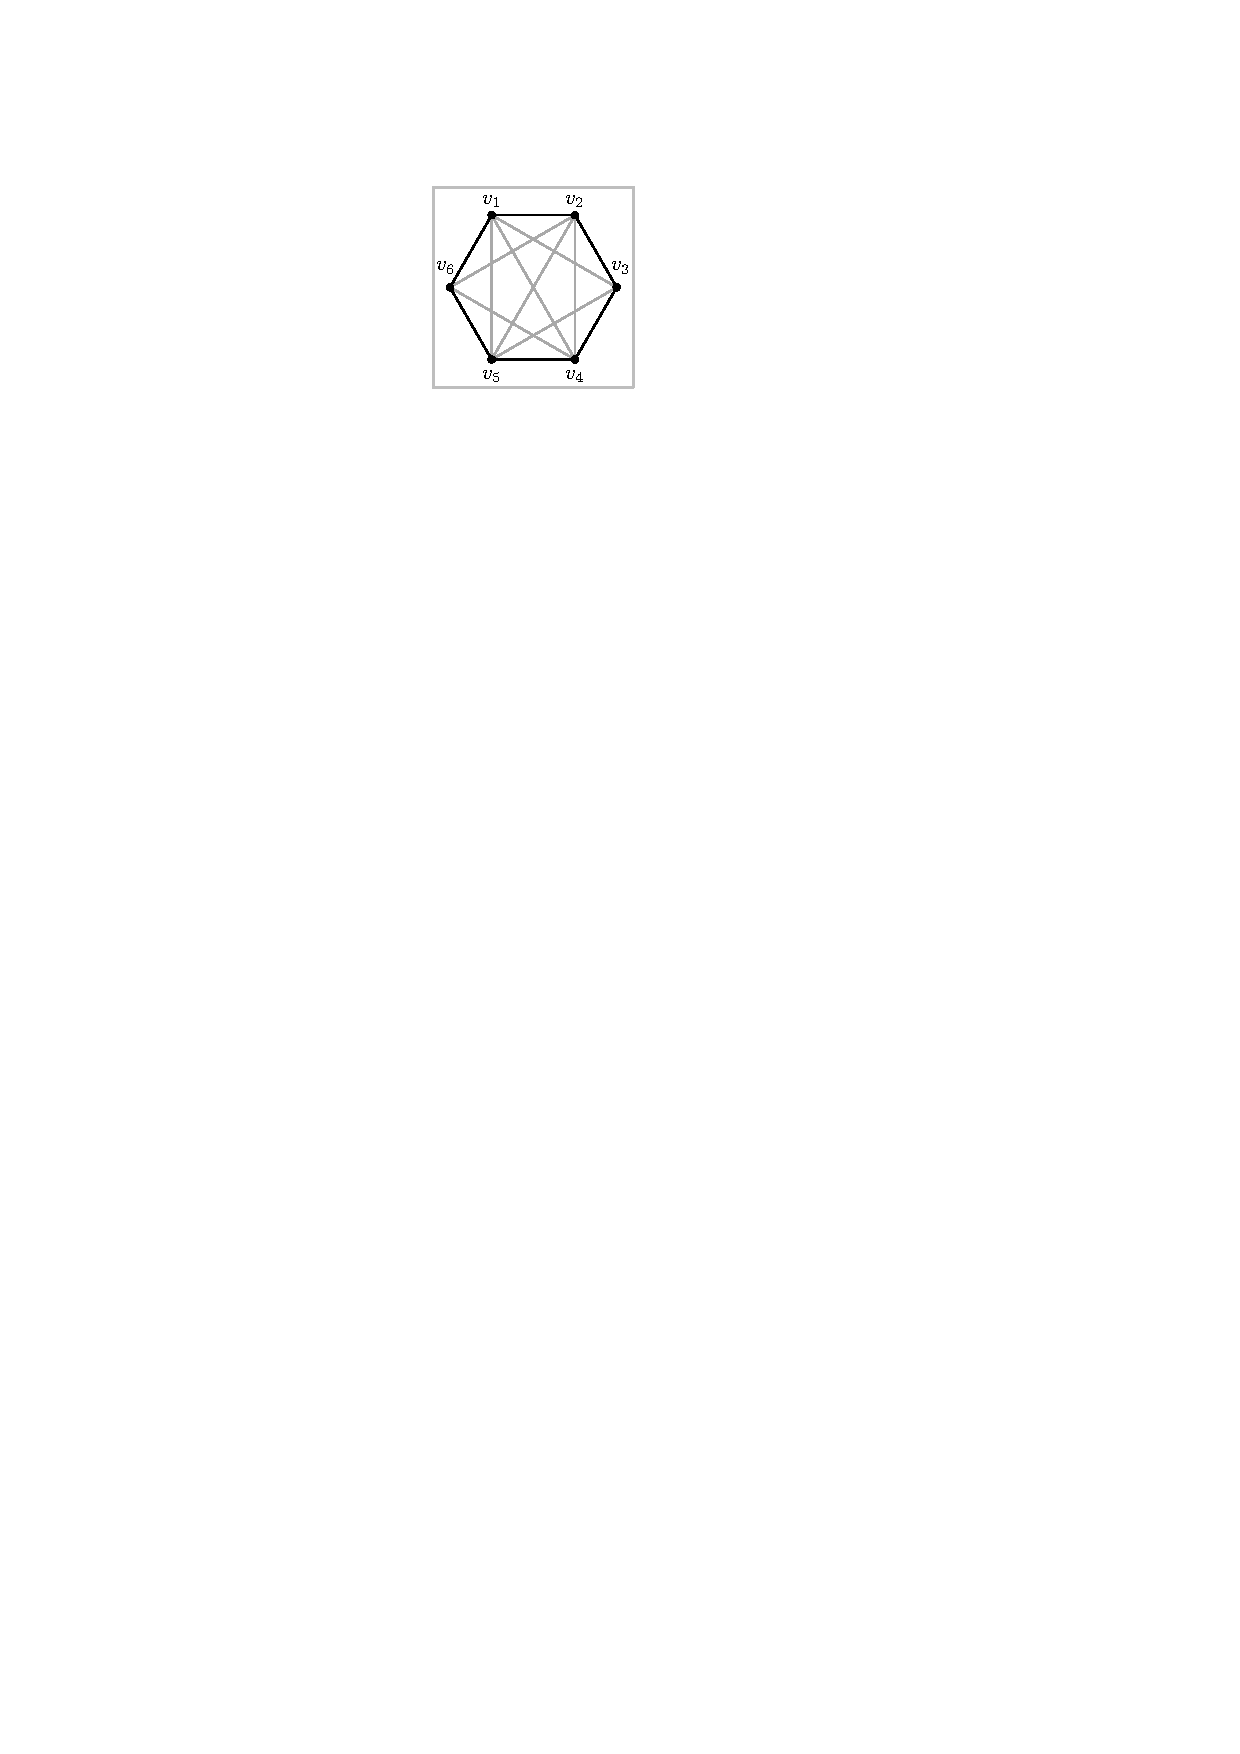
\includegraphics[width=\textwidth,page=1]{images/polygon_conf}
        \subcaption{~}\label{fig:6gon}
    \end{minipage}
    \begin{minipage}[b]{.16\textwidth}
        \centering
        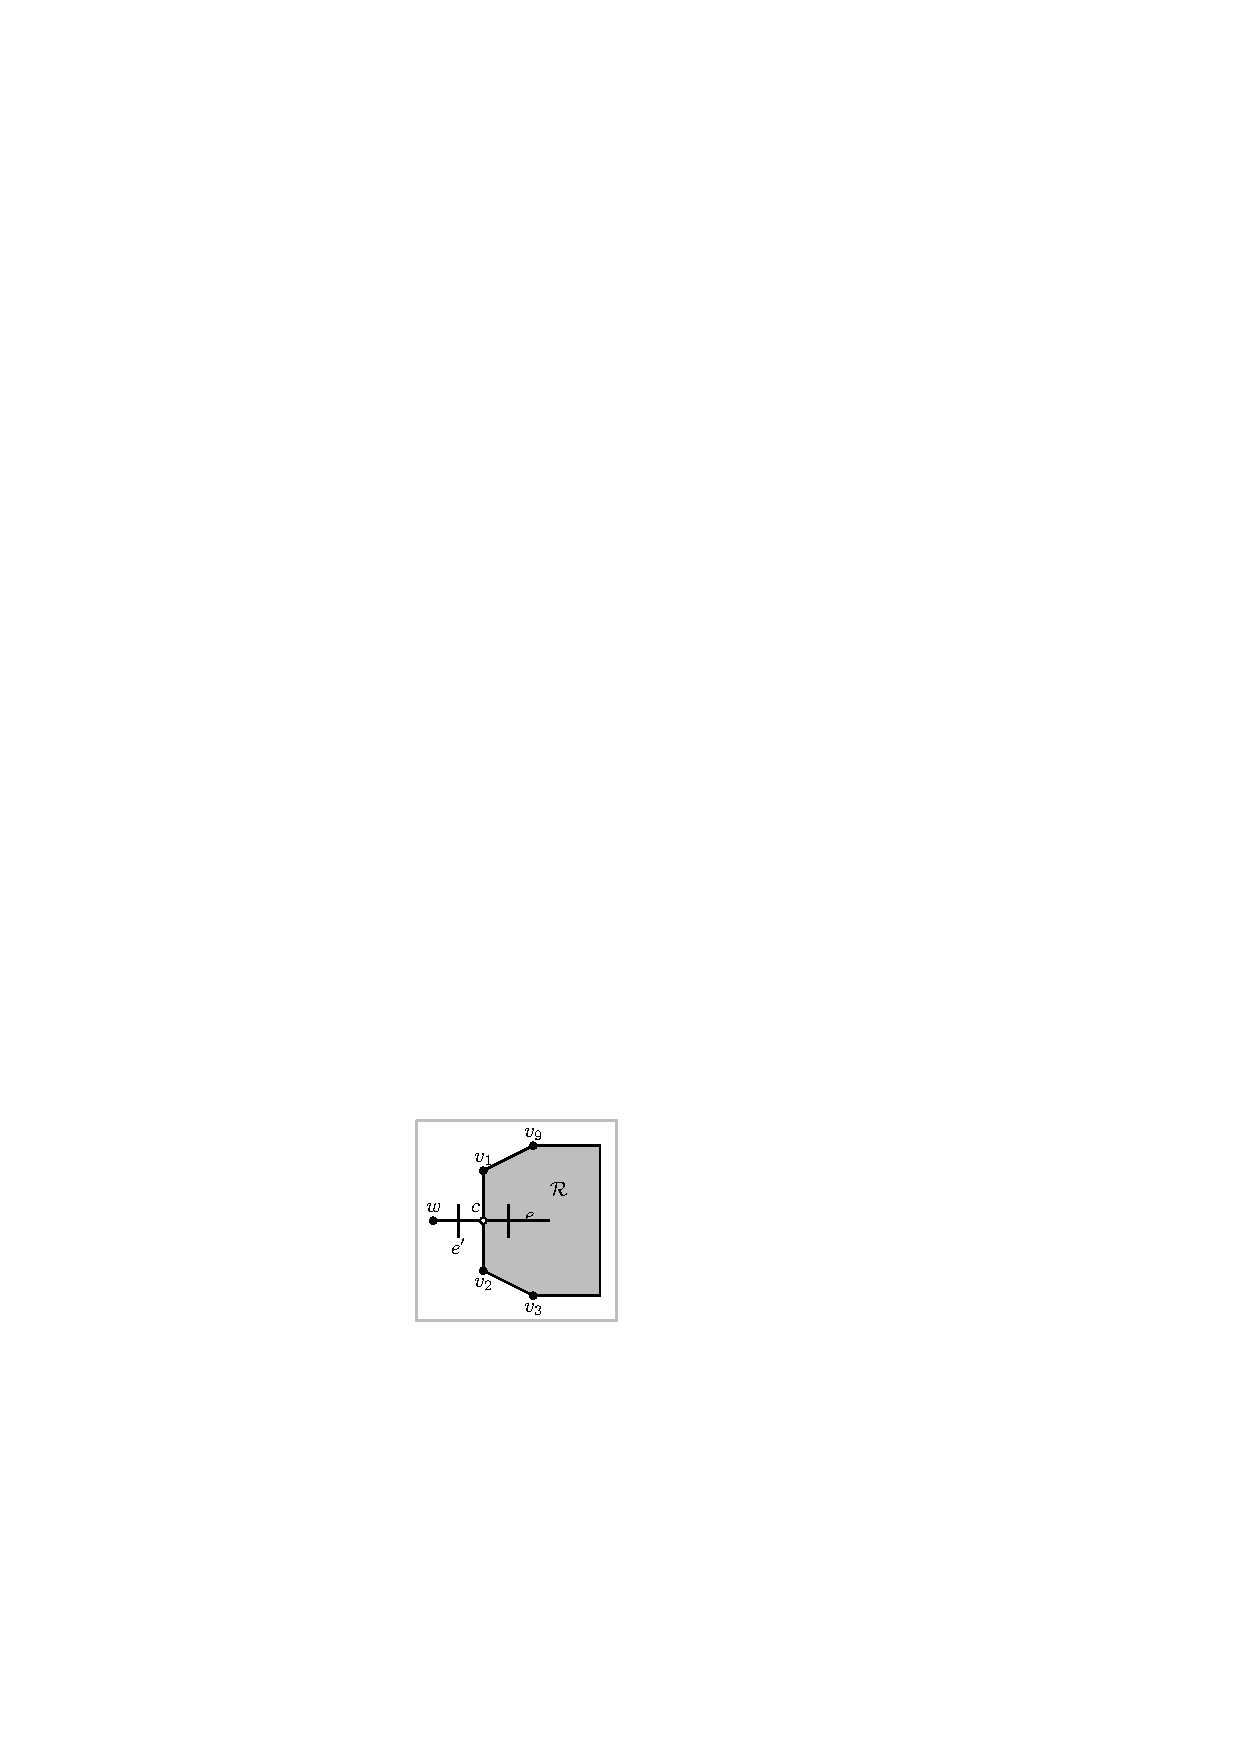
\includegraphics[width=\textwidth,page=1]{images/3planar_polygon}
        \subcaption{~}\label{fig:cs1}
    \end{minipage}
    \begin{minipage}[b]{.16\textwidth}
        \centering
        \includegraphics[width=\textwidth,page=2]{images/3planar_polygon}
        \subcaption{~}\label{fig:cs2}
    \end{minipage}
	\begin{minipage}[b]{.16\textwidth}
        \centering
        \includegraphics[width=\textwidth,page=3]{images/3planar_polygon}
        \subcaption{~}\label{fig:7_stick}
    \end{minipage}
    \begin{minipage}[b]{.16\textwidth}
        \centering
        \includegraphics[width=\textwidth,page=4]{images/3planar_polygon}
        \subcaption{~}\label{fig:cs_final}
    \end{minipage}
    \begin{minipage}[b]{.16\textwidth}
        \centering
        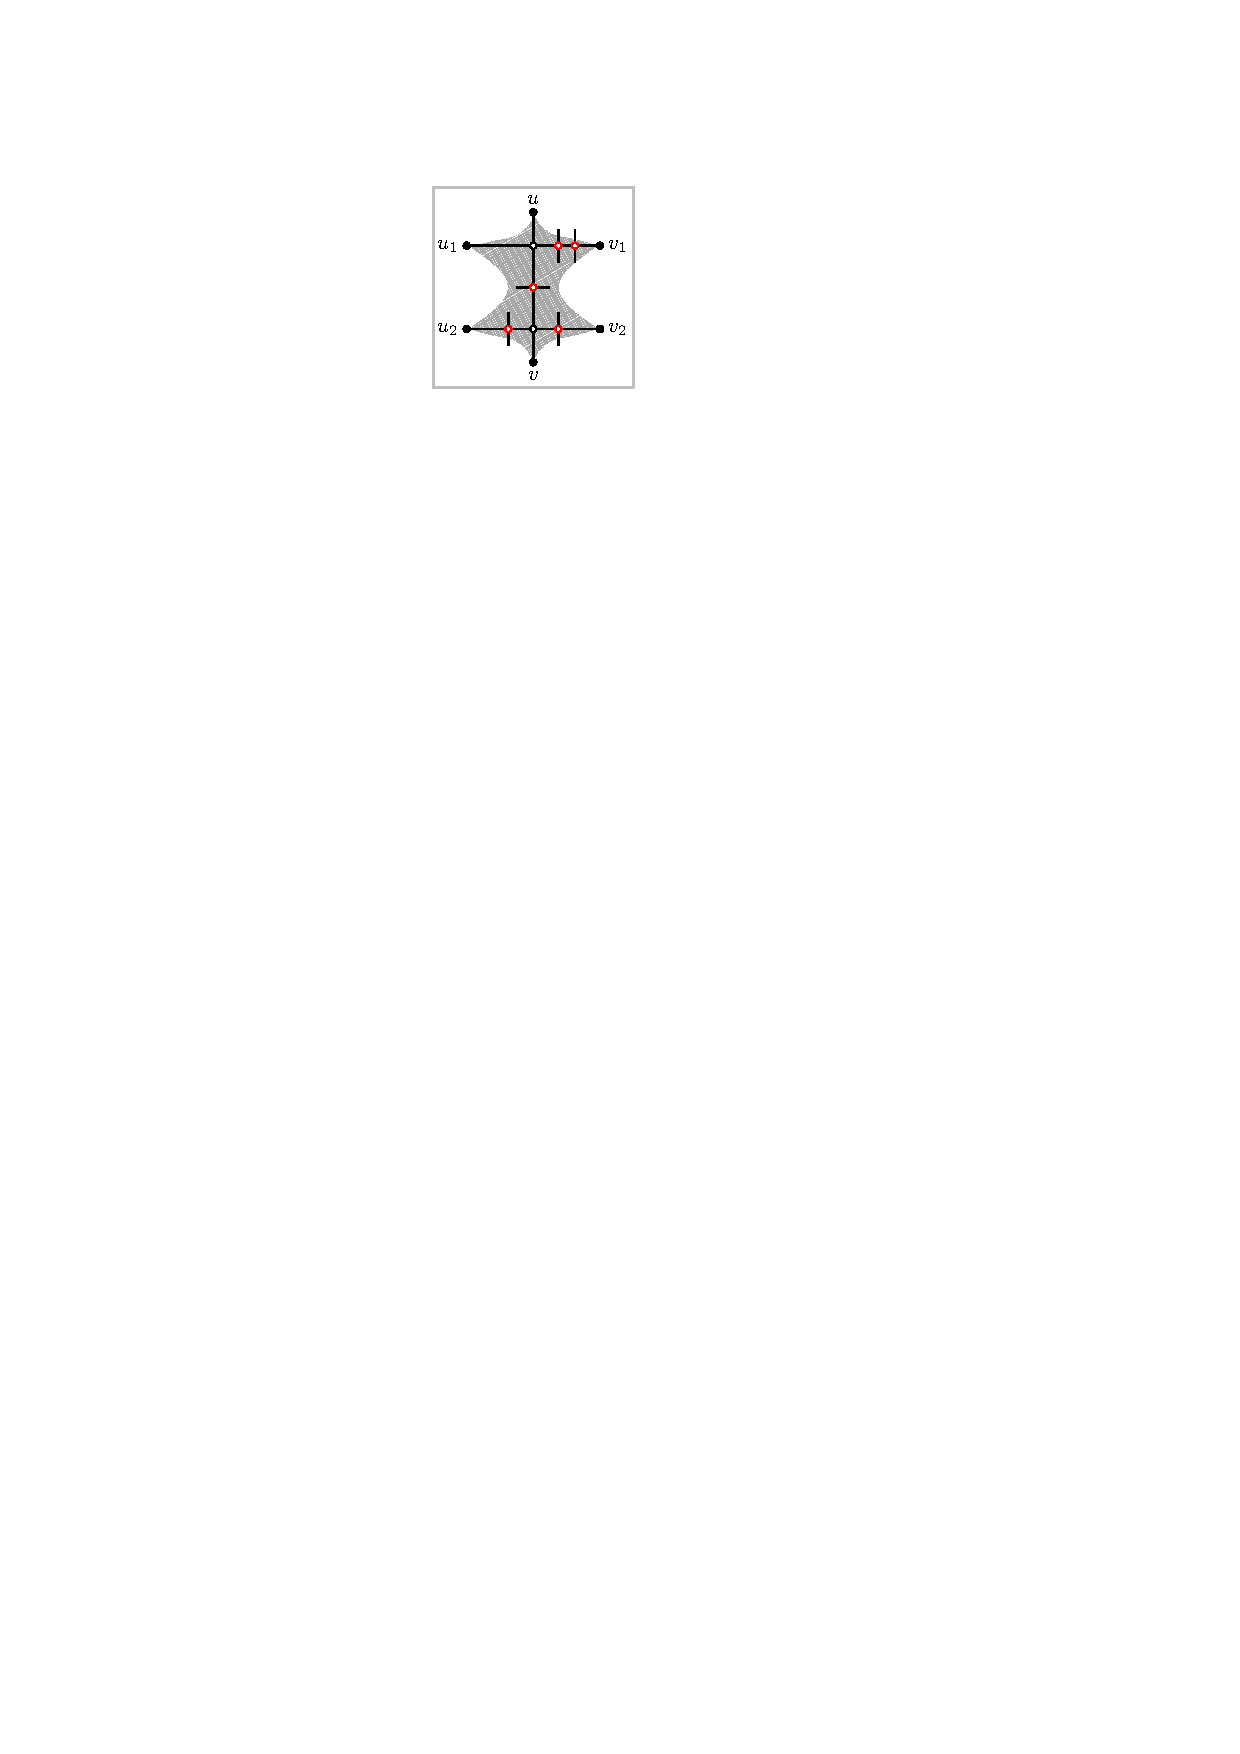
\includegraphics[width=\textwidth,page=1]{images/3planar_independent}
        \subcaption{~}\label{fig:independent}
    \end{minipage}
    \caption{%
    Different configurations used in  
    (a)~Lemma~\ref{lem:no-of-edges},
    (b)-(e)~Lemma~\ref{lem:size9}, 
    (f)~Lemma~\ref{lem:3_planar_independent}.}
    \label{fig:replacements_2}
\end{figure}

Recall that edge $e$ has one crossing in the interior of $\mathcal{C}$ (by Condition C.\ref{cnd:2} of the lemma) and one more crossing with edge $(v_1,v_6)$. By $3$-planarity, it follows that edge $e$ may have at most one more crossing, say with edge $e'$. Note that $e'$ may have an edge-segment in $E_{\mathcal{C}}$. Vertices $w,v_1,v_2,\dots,v_6$ define a \pp $\mathcal{C}'$ on $7$ vertices (see Figure~\ref{fig:cs2}). The set of passing-through segments $E_{\mathcal{C}'}$ of $\mathcal{C}'$ contains all edge-segments of $E_{\mathcal{C}}$ (that is, $E_{\mathcal{C}} \subseteq E_{\mathcal{C}'}$) plus at most two additional edge-segments: the one defined by edge $(v_1,v_6)$, and possibly an edge-segment of $e'$. Hence $|E_{\mathcal{C}'}| \leq 10$. 

\begin{claim}
All edges with an edge-segment in $E_{\mathcal{C}'}$ have at least one crossing in the interior of $\mathcal{C}'$.
\label{nclm:1}
\end{claim}
\begin{proof}
The claim clearly holds for all edge-segments of $E_{\mathcal{C}}$ (recall that $E_{\mathcal{C}}\subset E_{\mathcal{C}'}$). Since $(v_1,v_{6})$ and $e'$ both cross $e$ in the interior of $\mathcal{C}'$, it follows that the remaining edge-segments of $\mathcal{C}'$ (i.e., the ones defined by edges $(v_1,v_{6})$ and $e'$) have at least one crossing in the interior of $\mathcal{C}'$.
\end{proof}

\begin{claim}
At least one edge with an edge-segment in $E_{\mathcal{C}'}$ crosses one of the edges of $\mathcal{C}'$.
\label{nclm:2}
\end{claim}
\begin{proof}
Assume to the contrary that all edges with an edge-segment in $E_{\mathcal{C}'}$ do not cross $\mathcal{C}'$. Then, all edges with an edge-segment in $E_{\mathcal{C}'}$ can be drawn completely in the interior of $\mathcal{C}'$, which implies that all \pes of $\mathcal{C}'$ can be added in $\Gamma(G)$ (if they are not present already). This, however, contradicts Property~\ref{prp:3planar_odd_cycle}. 
\end{proof}

\noindent By Claim~\ref{nclm:2}, it follows that there exists an edge, say $g$, that crosses an edge of $\mathcal{C}'$. W.l.o.g.~assume that $g$ crosses $[w,v_1]$ of $\mathcal{C}'$.

\begin{claim}
All boundary edges of $\mathcal{C}'$ exist in $\Gamma(G)$
\label{nclm:3}
\end{claim}
\begin{proof}
In order to prove this claim, we remove from the interior of  $\mathcal{C}'$ all edges with an edge-segment in $E_{\mathcal{C}'}$ and replace them with the $10$ edges of the $3$-planar crossing pattern of Figure~\ref{fig:7_stick}. This allows us to add all boundary edges of  $\mathcal{C}'$ in $\Gamma(G)$ (if they are not present already). In addition, we can redraw the segment of $g$ in the interior of $\mathcal{C}'$ so that: % 
\begin{inparaenum}[(i)]
\item $g$ emanates from vertex $v_6$ of $\mathcal{C}'$,
\item $g$ crosses only \pe $[v_1,w]$ at point $c$, and
\item $g$ has no other crossings in the interior of  $\mathcal{C}'$.
\end{inparaenum}
Hence, $3$-planarity is preserved and the derived graph has at least as many edges as $G$. Since $G$ is optimal, it follows that all boundary edges of $\mathcal{C}'$ must exist in $\Gamma(G)$, which completes the proof of the claim.
\end{proof}

By Claim~\ref{nclm:3}, it follows that $g$ has one crossing in the interior of  $\mathcal{C}'$ and one more crossing with edge $(v_1,w)$ at point $c'$. We follow the same approach we used for expanding $\mathcal{C}$ (that has $6$ vertices) to $\mathcal{C}'$ (that has $7$ vertices). We can find an endpoint of $g$, say $z$, such that $w,z,v_1,v_2,\dots,v_6$ define a \pp $\mathcal{C}''$ on $8$ vertices. Furthermore, the set of passing-through segments $E_{\mathcal{C}''}$ of $\mathcal{C}''$ has at most $12$ elements (at most two more than $E_{\mathcal{C}'}$). We proceed by removing all edges with an edge-segment in $E_{\mathcal{C}''}$ and split $\mathcal{C}''$ into two true-planar cycles of length $6$ and $4$ respectively, by adding  true-planar chord $(v_1,v_6)$; refer to Figure~\ref{fig:cs_final}. In the interior of the $6$ cycle, we add the $8$ edges of the $3$-planar pattern of Figure~\ref{fig:6gon}. In the interior of the $4$-cycle, we add a vertex $x$ with a true planar edge $(v_1,x)$. Vertices $v_1,x,v_1,w,z,v_6$ define a new \pp on $6$ vertices, allowing us to add $8$ more edges in its interior. 

Summarizing the above, we removed at most $12$ edges, added a vertex and a total of $18$ edges. If $n$ and $m$ are the number of vertices and edges of $G$, then the derived graph $G'$ has $n'=n+1$ vertices and at least $m'\geq m+6$ edges. The last equation gives $m'\geq 5.5n'-10.5$, i.e. $G'$ has more edges than allowed; a contradiction.
\end{proof}

Let $(u,v)$ be an edge of $G$ that is crossed by two edges $(u_1,v_1)$ and $(u_2,v_2)$ in $\Gamma(G)$. By Property~\ref{prp:parallel} it follows that at least one of parallel edges $[u_1,u_2]$ and $[v_1,v_2]$ is a \pe of $\Gamma(G)$. Recall that in the case where both parallel edges $[u_1,u_2]$ and $[v_1,v_2]$ are \pes of $\Gamma(G)$, edges $(u_1,v_1)$ and $(u_2,v_2)$ are called independent.

\begin{lemma}\label{lem:3_planar_independent}
Let $\Gamma(G)$ be a PMCM $3$-planar drawing of an optimal $3$-planar graph~$G$. If edge $(u,v)$ is crossed by two independent edges $(u_1,v_1)$ and $(u_2,v_2)$, then $(u,v)$ is a chord of an empty true-planar $6$-cycle.
\end{lemma}
\begin{proof}
Refer to Figure~\ref{fig:independent}. Since $(u_1,v_1)$ and $(u_2,v_2)$ are independent edges, both parallel edges $[u_1,u_2]$ and $[v_1,v_2]$ are \pes. By Property~\ref{prp:corner}, it follows that corner edges $[u, u_1]$, $[u,v_1]$, $[u,u_2]$ and $[v,v_2]$ are also potential edges. Hence, vertices $u$, $u_1$, $u_2$, $v$, $v_2$ and $v_1$ define a \pp $\mathcal{C}$ on six vertices (gray-shaded in Figure~\ref{fig:independent}). Let $E$ be the set of passing-through edges of $\mathcal{C}$. We claim that $|E|\leq 8$. Indeed, set $E$ contains edges $(u,v)$, $(u_1,v_1)$, $(u_2,v_2)$, at most one other edge that crosses $(u,v)$, and at most four other edges that cross $(u_1,v_1)$ or $(u_2,v_2)$. We proceed by removing all edges of $E$ from $\Gamma(G)$ and replace them with the $3$-planar crossing pattern of Figure~\ref{fig:6gon}. In the derived drawing there exist $8$ edges that are drawn in the interior of $\mathcal{C}$ (without crossing $\mathcal{C}$). Since $G$ is optimal, it follows that $|E|=8$ and additionally all boundary edges of $\mathcal{C}$ exist in $\Gamma(G)$. Since $|E|=8$, all edges of $E$ have at least one crossing in the interior of $\mathcal{C}$. So, by Lemma~\ref{lem:size9} there exists an empty true-planar $6$-cycle that has $e$ as chord.
\end{proof}

We are now ready to state the main property of PMCM-drawings of optimal $3$-planar graphs. Recall that we denote by $\mathcal{X}(G)$ the crossing graph of $\Gamma(G)$ and by $\mathcal{X}(e)$ the crossing component of $\mathcal{X}(G)$ containing edge $e$ of $G$\todo{propaged set of crossings $\rightarrow$ crossing component, $S(e) \rightarrow \mathcal{X}(e)$, $C_G \rightarrow \mathcal{X}(G)$}.

\begin{lemma}\label{lem:3_planar_small_faces}
Let $\Gamma(G)$ be a PMCM $3$-planar drawing of an optimal $3$-planar graph $G$. Any edge that is crossed three times in  $\Gamma(G)$ is a chord of an \textcolor{blue}{empty true-planar $6$-cycle in $\Gamma(G)$.}%, where $6\leq s\leq 9$. 
\end{lemma}
\begin{proof}
%Recall that if $e$ is a chord of a true-planar $s$-cycle that has no vertices in its interior, then all edges of $\mathcal{X}(e)$ are also chords of this $s$-cycle

Let $e=(u,v)$ be an edge of $G$ that crosses with edges $e_i=(u_i,v_i)$ in $\Gamma(G)$, for $i=1,2,3$. Consider the crossing component $\mathcal{X}(e)$ where $e$ belongs to. We distinguish two cases depending on whether there exists an edge in $\mathcal{X}(e)$ that crosses with two independent edges or not.

Suppose that this is the case, and an edge of $\mathcal{X}(e)$ is crossed by two independent edges. Then by Lemma~\ref{lem:3_planar_independent}, there exists an empty true-planar $s$-cycle (without vertices in its interior) defining a \pp with this edge as a chord. Then all edges of $\mathcal{X}(e)$ are also drawn as chords of the $s$-cycle and the lemma follows.

Assume, now that all edges of $\mathcal{X}(e)$ with at least two crossings, are not crossed by independent edges in $\Gamma(G)$. Then, for edge $e$, that crosses with edges $e_1$, $e_2$, and $e_3$, we have that edges $e_i$, $e_j$ ($1\leq i<j\leq 3$) are not parallel edges. This implies that exactly one of parallel edges $[u_i,u_j]$ or $[v_i,v_j]$ is not a \pe. For the sake of simplicity let's refer to parallel edges $[u_i,u_j]$ and $[v_i,v_j]$ as the ``$u$-parallel edge'' and ``$v$-parallel edge'' respectively of $e_i$ and $e_j$. 
There are three ways to combine indices $i$ and $j$ and for every combination exactly one of the ``$u$-parallel edge'' and ``$v$-parallel edge'' is not a \pe. This implies that: there exist at least two combinations such that their ``$u$-parallel edges'' are not \pes, or there exist at least two combinations such that their ``$v$-parallel edges'' are not \pes of $\Gamma(G)$. W.l.o.g. assume that there exist two combinations of indices, say $i_1$ with $j_1$ and $i_2$ with $j_2$ for which their ``$u$-parallel edges'', namely $[u_{i_1},u_{j_1}]$ and $[u_{i_2},u_{j_2}]$  are not \pes. It is clear that since $i_1\neq j_1$, $i_2\neq j_2$ and $\left\{i_1,i_2,j_1,j_2\right\}\subseteq\left\{1,2,3\right\}$, at least two indices are the same. W.l.o.g. assume that $i_1=i_2$; other cases are symmetric. Let $i=i_1=i_2$. Then we have that parallel edges  $(u_i,u_{j_1})$ and $(u_i,u_{j_2})$ are not \pes, where $j_1\neq j_2$. This implies that $u_i=u_{j_1}$ and $u_i=u_{j_2}$. It is not hard to see that parallel edge $(u_{j_1},u_{j_2})$ can not be a \pe either; for an example see Figure~\ref{fig:3_planar_small_faces_example}, where $i=1$. This implies that for any combination of idices $i$ and $j$, parallel edge $[u_i,u_j]$ is not a \pe. Hence, for any edge of $\mathcal{X}(e)$ with three crossings in $\Gamma(G)$, we have the crossing pattern of Figure~\ref{fig:3_planar_small_faces_conf}, where the grey-shaded region has no vertices in its interior.

%Since there are three pairs of potential parallel edges $e_i$ and $e_j$, there exist at least two pairs, say $e_i$-$e_j$ and $e_{i'}$-$e_{j'}$ for which both \pes $(u_i,u_j)$ and $(u_{i'},u_{j'})$, or both \pes $(v_i,v_j)$ and $(v_{i'},v_{j'})$ do not exist. Assume w.l.o.g. that edges $(u_i,u_j)$ and $(u_{i'},u_{j'})$ do not exist. Since $1\leq i,i',j,j'\leq 3$ and $i\neq j$, $i'\neq j'$, we can also assume that $i=i'$. Then we have that potential parallel edges  $(u_i,u_j)$ and $(u_i,u_{j'})$ do not exist. This implies that $u_i=u_j$ and $u_i=u_j'$. Also, the potential parallel edge $(u_j,u_{j'})$ can not exist, since otherwise at least one of potential parallel edges $(u_i,u_j)$ or $(u_i,u_{j'})$ would also exist (for an example refer to Figure~\ref{fig:3_planar_small_faces_example}, where $i=1$). Hence, for any edge of $S(e)$ with three crossings in $\Gamma(G)$, we have the crossing pattern of Figure~\ref{fig:3_planar_small_faces_conf}, where the grey-shaded region has no vertices in its interior.

So far, vertices $u,v_1,v_2,v_3,v,u_1$ define a \pp $\mathcal{C}_6$ on six vertices. We want to apply Lemma~\ref{lem:size9} for $s=6$, and to achieve this, we claim that there exist at most $8$ edges that pass through the interior of $\mathcal{C}_6$ and satisfy Conditions C.1 and C.2 of the lemma, and also that all boundary edges of $\mathcal{C}_6$ belong in $\Gamma(G)$. We claim that any edge crossing $e_2$ must also cross $e_1$ or $e_3$. In order to prove the claim, suppose that there exists an edge $e'=(u',v')$ that crosses with $e_2$ in the interior of $\mathcal{C}_6$. Since $e_2\in \mathcal{X}(e)$, $e_2$ is not crossed by independent edges. So, edges $e'=(u',v')$ and $e=(u,v)$ are not independent edges, and exactly one of parallel edges $[u,u']$ or $[v,v']$ is not a \pe. Assume w.l.o.g. that parallel edge $[u,u']$ is not a \pe. This implies that $u=u'$ and that the region $R$ \todo{use the notation of preliminaries}defined by edges $e_2$, $e$ and $e'$ has no vertices in its interior (see Figure~\ref{fig:3_planar_small_faces_conf_middle_a}). Then, $e'$ must cross with $e_1$, as otherwise vertex $v_1$ would be in the interior of $R$; see Figure~\ref{fig:3_planar_small_faces_conf_middle_b}. Hence, any edge that crosses with $e_2$, must also cross with $e_1$ or $e_3$ as claimed. 

The above claim assures that there exist at most four other edges that pass through the interior of $\mathcal{C}_6$ and cross with edges $e_1$, $e_2$ or $e_3$, i.e. we have at most $8$ edges that pass through the interior of $\mathcal{C}_6$. We proceed by removing edges $e$, $e_i$ and all edges that cross with edges $e_i$ in  $\mathcal{C}_6$ ($i=1,2,3$), and replace them with the $3$-planar pattern of Figure~\ref{fig:6gon}. The derived graph has at least as many edges as $G$, and since $G$ is optimal, the boundary edges of $\mathcal{C}_6$ belong in the drawing $\Gamma(G)$. So, the vertices of $\mathcal{C}_6$ define an empty $6$-cycle in $\Gamma(G)$, and the set $E_{\mathcal{C}}$ of passing-through edge-segments of $\mathcal{C}_6$ has size $|E_{\mathcal{C}}|=8$ (Condition C.1). Furthermore, every edge-segment of $E_{\mathcal{C}}$ has at least one crossing in the interior of $\mathcal{C}_6$ (Condition C.2). By Lemma~\ref{lem:size9}, %for $s=6$, we have that $e$ is a chord of a true planar $s'$-cycle for $6\leq s'\leq 9$.
\textcolor{blue}{we have that $e$ is a chord of a true planar $6$-cycle.}
\end{proof}

\begin{figure}[htb]
    \centering
    \begin{minipage}[b]{.24\textwidth}
        \centering
        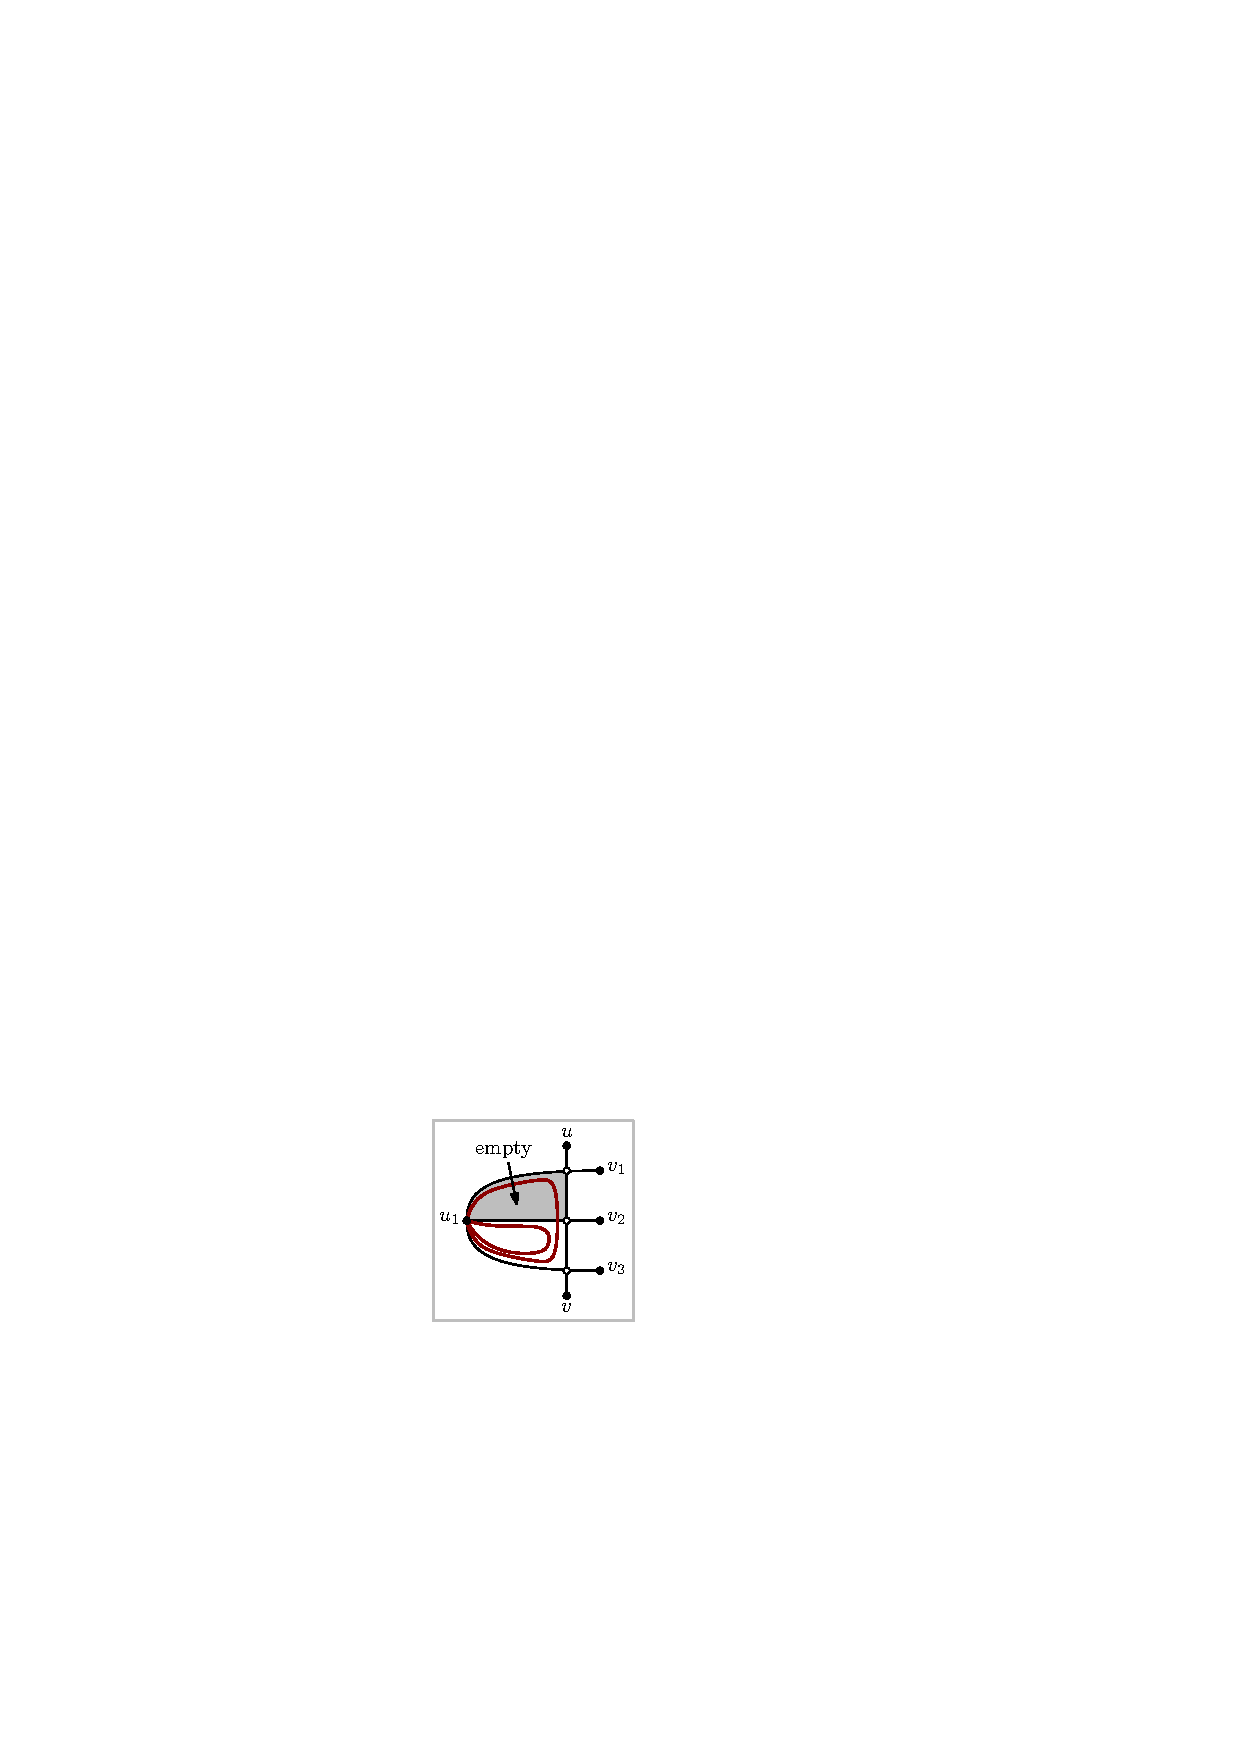
\includegraphics[width=\textwidth,page=1]{images/3planar_small_faces}
        \subcaption{~}\label{fig:3_planar_small_faces_example}
    \end{minipage}
    \begin{minipage}[b]{.24\textwidth}
        \centering
        \includegraphics[width=\textwidth,page=2]{images/3planar_small_faces}
        \subcaption{~}\label{fig:3_planar_small_faces_conf}
    \end{minipage}
    \begin{minipage}[b]{.24\textwidth}
        \centering
        \includegraphics[width=\textwidth,page=3]{images/3planar_small_faces}
        \subcaption{~}\label{fig:3_planar_small_faces_conf_middle_a}
    \end{minipage}
		\begin{minipage}[b]{.24\textwidth}
        \centering
        \includegraphics[width=\textwidth,page=4]{images/3planar_small_faces}
        \subcaption{~}\label{fig:3_planar_small_faces_conf_middle_b}
    \end{minipage}
    \caption{%
    (a):~If the parallel edge $[u_1,u_1]$ is a\pe for edges $(u_2,v_2)$ and $(u_3,v_3)$ then it is also a \pe for edges $(u_1,v_1)$ and $(u_3,v_3)$.  (b)-(d):~Configuration of Lemma~\ref{lem:3_planar_small_faces}.}
    \label{fig:3_planar_small_faces}
\end{figure}

By Lemma~\ref{lem:3_planar_small_faces}, we have that any edge of $G$ that is crossed three times in $\Gamma(G)$ is a chord of an empty true-planar %$s$-cycle for $6\leq s\leq9$. 
\textcolor{blue}{$6$-cycle}. So, it remains to consider edges of $G$ that have at most two crossings in $\Gamma(G)$, i.e. crossing components where every edge has at most two crossings. Note that we can not use directly  Lemma~\ref{lem:2_planar_small_faces}, since its proof is based on the fact that optimal $2$-planar graphs have at most $5n-10$ edges, however, we can formulate its \textcolor{red}{analogue lemma as follows:} \textcolor{blue}{proof and get the following result:}
\begin{lemma}
Let $\Gamma(G)$ be a PMCM $3$-planar drawing of an optimal $3$-planar graph $G$. Let $\mathcal{X}$ be a crossing component. \textcolor{blue}{Then there is at least one edge in $\mathcal{X}$ that has three crossings.}
\label{lem:3_planar_small_faces_2}
\end{lemma}
%\begin{lemma}
%Let $\Gamma(G)$ be a PMCM $3$-planar drawing of an optimal $3$-planar graph $G$. Let $\mathcal{X}$ be a crossing component where every edge has at most two crossings. Then edges of $\mathcal{X}$ are chords of a true-planar $5$-cycle in $\Gamma(G)$, that contains no vertices in its interior. 
%\label{lem:3_planar_small_faces_2}
%\end{lemma}
\begin{proof}
\textcolor{blue}{For a proof by contradiction, suppose that there exists a crossing component $\mathcal{X}$ where all edges have at most two crossings.}
We distinguish two cases depending on whether $\mathcal{X}$ contains an edge with two crossings or not. Suppose first that this is not the case. Then all edges of $\mathcal{X}$ have at most one crossing. Let $e\in \mathcal{X}$ crossing with $e'\in \mathcal{X}$. Clearly $\mathcal{X}=\left\{e,e'\right\}$. The four endpoints of edges $e$ and $e'$ define a \pp $\mathcal{C}_4$ on $4$ vertices, as in Figure~\ref{fig:3_planar_one_crossing_before} and there are no other edges passing through the interior of $\mathcal{C}_4$. We proceed by removing edges $e$ and $e'$ and replace them with the $3$-planar pattern of Figure~\ref{fig:3_planar_one_crossing_after}. The derived graph $G'$ has $n'=n+1$ vertices and $m'=m-2+8$ edges, where $n$ and $m$ are the number of vertices and edges of $G$ respectively. Then, $G'$ is $3$-planar and has $m'=5.5n'-10.5>5.5n'-11$ edges; a contradiction to the optimality of $G$.

Now, assume that there exists an edge $e\in \mathcal{X}$, where $e=(u,v)$ crossing with two edges $e_1=(u_1,v_1)$ and $e_2=(u_2,v_2)$. By Lemma~\ref{lem:3_planar_independent} edges $e_1$ and $e_2$ are not independent edges. \textcolor{blue}{Following the proof of Lemma~\ref{lem:2_planar_small_faces}, the endpoints of $(u,v)$, $(u',v')$ and $(u'',v'')$ define a \pp $\mathcal{C}$ on five vertices, with at most five edges passing through its interior. We can alter $G$, by redrawing the five edges passing through the interior of $\mathcal{C}$ so that $\mathcal{C}$ contains five chords and all its boundary edges are true-planar in the new drawing. Then the derived graph is optimal, since it has at least as many edges as $G$, but $\mathcal{C}$ is a true-planar $5$-cycle; a contradiction to Property~\ref{prp:3planar_even_order}.}


%Following the proof of Lemma~\ref{lem:2_planar_small_faces} we can find:
%\begin{enumerate}
%\item  a \pp on five vertices whose boundary edges define a true planar $5$-cycle with $e$ as a chord, or,
%\item a \pp $\mathcal{C}_6$ on six vertices with at most $6$ edges passing through its interior. In this case, we remove all edges with an edge-segment in the set of passing-through segments of $\mathcal{C}_6$ and use the $3$-planar pattern of Figure~\ref{fig:6gon} that gives $8$ edges in drawn in the interior of $\mathcal{C}_6$. The derived graph clearly has more edges than $G$, contradicting its optimality.
%\end{enumerate}
\end{proof}

\begin{figure}[htb]
    \centering
    \begin{minipage}[b]{.24\textwidth}
        \centering
        
\includegraphics[width=\textwidth,page=1]{images/3planar_one_crossing}
        \subcaption{~}\label{fig:3_planar_one_crossing_before}
    \end{minipage}
    \begin{minipage}[b]{.24\textwidth}
        \centering
        
\includegraphics[width=\textwidth,page=2]{images/3planar_one_crossing}
        \subcaption{~}\label{fig:3_planar_one_crossing_after}
    \end{minipage}
		%\begin{minipage}[b]{.24\textwidth}
        %\centering
        %
\includegraphics[width=\textwidth,page=3]{images/3planar_one_crossing}
        %\subcaption{~}\label{fig:3_planar_triangle}
    %\end{minipage}
    \caption{%
    Configurations used in Lemma~\ref{lem:3_planar_small_faces_2}.}.
    \label{fig:3_planar_one_crossing_1}
\end{figure}

%\begin{lemma}
%Let $\Gamma(G)$ be a PMCM $3$-planar drawing of an optimal $3$-planar graph $G$. There is no true planar $3$-cycle without vertices in its interior. 
%\label{lem:3_planar_triangle}
%\end{lemma}
%\begin{proof}
%Suppose that there exists a true planar $3$-cycle in $\Gamma(G)$ without vertices in its interior. Then we can add a vertex in the interior of this cycle, and $6$ edges by using the $3$-planar pattern of Figure~\ref{fig:3_planar_triangle}. The derived graph $G'$ has $n'=n+1$ vertices and $m'=m+6$ edges, where $n$ and $m$ are the number of vertices and edges of $G$ respectively. Then, $G'$ is $3$-planar and has $m'=5.5n'-10.5>5.5n'-11$ edges; a contradiction.
%\end{proof}

%Now we are ready to prove the main property of every PMCM-drawing $\Gamma(G)$ of a maximal $3$-planar graph. 

Lemma~\ref{lem:3_planar_small_faces_2} states that any crossing component $\mathcal{X}$  contains at least one edge with three crossings, and by Lemma~\ref{lem:2_planar_small_faces} all edges of $\mathcal{X}$ are drawn as chords of a true-planar $6$-cycle. Also, similarly with the case of PMCM-drawings  of optimal $2$-planar graphs, one can prove that the true planar skeleton $\Pi(G)$ is connected. Therefore, we have proven the following:
%Lemma~\ref{lem:3_planar_small_faces_2} states that if in a crossing component $\mathcal{X}$ all edges have at most two crossings, then there exists a true-planar $5$-cycle in $\Gamma(G)$. However this contradicts Property~\ref{prp:3planar_odd_cycle}. Hence, $\mathcal{X}$ contains at least one edge with three crossings, and by Lemma~\ref{lem:2_planar_small_faces} all edges of $\mathcal{X}$ are drawn as chords of a true-planar $s$-cycle for $6\leq s\leq 9$. Again by Property~\ref{prp:3planar_odd_cycle} $s$ must be even, i.e. $s=6$ or $8$. Also, similarly with the case of PMCM-drawings  of optimal $2$-planar graphs, one can prove that the true planar skeleton $\Pi(G)$ is connected. Therefore, we have proven the following:
 

%By combining Lemmas~\ref{lem:3_planar_small_faces}, \ref{lem:3_planar_small_faces_2} and \ref{lem:3_planar_triangle} the following is straightforward:
 
%\begin{corollary}\label{cor:3_planar_faces_general}
%The true planar structure $\Pi(G)$ of a PMCM $3$-planar drawing of an optimal $3$-planar graph $G$ contains faces of length $6$ or $8$.
%\end{corollary}

\begin{corollary}\label{cor:3_planar_faces_general}
The true planar structure $\Pi(G)$ of a PMCM $3$-planar drawing of an optimal $3$-planar graph $G$ contains faces of length $6$.
\end{corollary}


 %\begin{corollary}\label{cor:3_planar_faces_general}
%The true planar structure $\Pi(G)$ of a PMCM $3$-planar drawing of an optimal $3$-planar graph $G$ on $n$ vertices contains faces of length at least $6$ and at most $9$.
%\end{corollary}
 %Now we are ready to prove the main property of  PMCM $3$-planar drawings of optimal $3$-planar graphs.
 %
 %\begin{lemma}\label{lem:3_planar_faces_final}
  %The true planar structure $\Pi(G)$ of a PMCM $3$-planar drawing of an optimal $3$-planar graph $G$ on $n$ vertices contains only faces of length $6$.
 %\end{lemma}
%
 %\begin{proof}
  %Let $m_{p}$ and $m_c$ be the total number of true planar and crossing edges of $G$ in any PMCM $3$-planar drawing $\Gamma(G)$. 
	%Clearly, $m_p+m_c=m$ where $m$ is the number of edges of $G$.
	%By Euler's formula we have that  
  %\begin{equation}
	%\label{eq:euler}
   %m_{p}+2=n+f\Rightarrow m_p-f=n-2
  %\end{equation}
  %%
	%where $f$ is the total number of faces of $\Pi(G)$. Let $f_s$ be the number of faces of $\Pi(G)$ of length $s$. By Corollary~\ref{cor:3_planar_faces_general} we have that $s=6$ or $s=8$. Hence $f=f_6+f_8$. 
	%Also, by counting the edges of all faces of $\Pi(G)$ we have that
  %\begin{equation}
	%\label{eq:faces}
   %2m_{p}=6f_6+8f_8\Rightarrow m_p=3f+f_8\Rightarrow m_p-f=2f+f_8\Rightarrow f=(m_p-f-f_8)/2
  %\end{equation}
%%
  %On the other hand for the number of crossing edges $m_c$, by Lemma~\ref{lem:no-of-edges} we obtain  
  %\begin{equation}
	%\label{eq:crossing}
   %m_{c}=8f_6+11f_8=8f+3f_8
  %\end{equation}
%%
  %Hence, for the total number of edges of $G$ we have 
	%%\todo{rewrite the equations}
  %
	%$\begin{array}{ll}
   %m& =m_{p}+m_{c}\stackrel{(\ref{eq:faces}), (\ref{eq:crossing})}{=}(3f+f_8)+(8f+3f_8)=11f+4f_8\\
		%& \stackrel{(\ref{eq:faces})}{=}11(m_p-f-f_8)/2+4f_8=11(m_p-f)/2-3f_8/2\\
    %& \stackrel{(\ref{eq:euler})}{=}11(n-2)/2-3f_8/2\leq 11(n-2)/2
  %\end{array}$
%%
  %%$\begin{array}{ll}
   %%|E(G)|= & 5.5n-11\\
    %%\Rightarrow &m_{p}+m_{c}= 5.5n-11\\
    %%\Rightarrow &m_{p}+m_{c}= 5.5(m_{p}-f)\\
    %%\Rightarrow &2m_{c}= 9m_{p}-11f\\
    %%\Rightarrow &10s_5+16s_6+18s_7+22s_8+28s_9 = 4.5(5s_5+6s_6+7s_7+8s_8+9s_9)\\
   %%&-11(s_5+s_6+s_7+s_8+s_9)\\
    %%\Rightarrow &10s_5+16s_6+18s_7+22s_8+28s_9=11s_5+16s_6+20.5s_7+25s_829.5s_9\\
    %%\Rightarrow &0= s_5+2.5s_7+3s_8+1.5s_9\\
   %%\Rightarrow &0=s_5=s_7=s_8=s_9
  %%\end{array}$
%Since $G$ is optimal $m=11(n-2)/2=5.5n-11$ must hold. 
%The last equality implies that $f_8=0$ and there are only faces of length $6$ in the true planar structure $\Pi(G)$.
 %\end{proof}

%Recall that at the beginning of this section we made the assumption that $\Gamma(G)$ is almost-simple, i.e. there is no pair of edges that cross twice in the drawing $\Gamma(G)$. In the following, we prove that in any PMCM drawing of an optimal $3$-planar graph $G$ on $n$ vertices there are no such pairs of edges.
 %By Lemma~\ref{lem:2_planar_faces} we can characterize all maximal $2$-planar graphs. Since the true planar subgraph of such a graph contains only faces of length $5$, we can start with a $5$-tiling of the plane. Now in the interior of every face of length $5$, we can add all  $5$ missing edges.



%By combining Lemma~\ref{lem:3_planar_faces_final} and Property~\ref{prp:3_planar_cross_twice}, we can characterize all optimal $3$-planar graphs:


 %By Property~\ref{prp:3_planar_cross_twice} we have that Lemma~\ref{lem:3_planar_faces_final} holds for all maximal $3$-planar graphs. 
Since the true planar subgraph of such a graph contains only faces of length $6$, we can start with a $6$-tiling of the plane\todo{rephrase}. Now in the interior of every face of length $6$, we can add all  $8$ missing edges using the $3$-planar pattern of Figure~\ref{fig:6gon}.
%

